\documentclass[11pt]{article}

% ---------- packages ----------
\usepackage[a4paper,margin=1in]{geometry}
\usepackage{amsmath,amssymb,mathtools}
\usepackage{siunitx}
\usepackage[version=4]{mhchem}
\usepackage{booktabs}
\usepackage{microtype}
\usepackage{xcolor}
\usepackage[most]{tcolorbox}
\usepackage{enumitem}
\usepackage{titlesec}
\usepackage{tikz}
\usetikzlibrary{arrows.meta,positioning,shapes.geometric,fit,backgrounds,calc}
\usepackage[colorlinks=true,linkcolor=accent,citecolor=accent,urlcolor=accent]{hyperref}

% ---------- style ----------
\definecolor{accent}{HTML}{A8682F}
\definecolor{ink}{HTML}{222222}
\definecolor{lightaccent}{HTML}{F3E9DF}
\color{ink}

\titleformat{\section}{\Large\bfseries\color{ink}}{\thesection}{0.6em}{}[{\color{accent}\titlerule[1pt]}]
\titleformat{\subsection}{\large\bfseries\color{accent}}{\thesubsection}{0.5em}{}
\titlespacing*{\section}{0pt}{1.4em}{0.6em}

\newtcolorbox{keybox}[1][]{colback=lightaccent,colframe=accent,boxrule=0.6pt,
  arc=2pt,left=8pt,right=8pt,top=6pt,bottom=6pt,#1}

\newcommand{\R}{\mathcal{R}}
\newcommand{\nv}{\mathbf{n}}
\newcommand{\uv}{\mathbf{u}}
\newcommand{\jv}{\mathbf{j}}
\newcommand{\xv}{\mathbf{x}}
\newcommand{\Da}{\mathrm{Da}}
\newcommand{\Sh}{\mathrm{Sh}}
\newcommand{\Rey}{\mathrm{Re}}
\newcommand{\Prn}{\mathrm{Pr}}
\newcommand{\Sc}{\mathrm{Sc}}
\newcommand{\Pe}{\mathrm{Pe}}
\newcommand{\Kn}{\mathrm{Kn}}
\newcommand{\Gr}{\mathrm{Gr}}
\sisetup{detect-all}

% ---------- title ----------
\title{\vspace{-1.2cm}\textbf{A Physics-Informed Surrogate \& Optimization Pipeline\\ for Surface-Limited Si/Si Epitaxy in an RP-CVD Reactor}\\[2pt]
\large\normalfont\color{accent} Flow $+$ Heat Transfer $+$ Finite-Rate Surface Chemistry in CFD-ACE+}
\author{Prepared for M.\ — internal working roadmap}
\date{\today}

\begin{document}
\maketitle
\vspace{-0.6cm}

\begin{keybox}
\textbf{One-paragraph thesis.} You do not need a monolithic black box, and you should not start there. In the surface-reaction-limited, steady, laminar, dilute regime you have specified, the multiphysics \emph{factorizes}: the flow and thermal fields decouple from chemistry, the precursor field becomes a passive scalar with a weakly reactive wall, and the stiff surface kinetics collapse to a \emph{smooth, steady-state} input--output map. This lets you build a \textbf{hierarchical, mostly-physical surrogate} --- a differentiable two-resistance backbone, corrected by a small amount of ACE+ data --- that is far cheaper, more extrapolable, and more interpretable than Latin-hypercube black-boxing. Pure LHS sampling is kept only as a fallback and as an independent validator. The document below organizes this into a tiered pipeline with the math made explicit, then layers optimization (gradient/adjoint on the backbone, Bayesian optimization for the global Pareto front) on top.
\end{keybox}

\section{Problem statement and what we are allowed to exploit}

You are simulating Si homo-epitaxy in a reduced-pressure CVD (RP-CVD) reactor with three coupled ACE+ modules: \emph{Flow} (multicomponent momentum + species transport), \emph{Heat Transfer}, and \emph{Chemistry} restricted to \emph{finite-rate surface reactions} (no volumetric/gas-phase chemistry). The deliverables are (i) a \textbf{surrogate} $\widehat{\mathcal{Q}}(\theta;\,g)$ that predicts process quality of interest (QoI) $\mathcal{Q}$ --- growth rate, within-wafer uniformity, precursor utilization, selectivity --- as a function of operating point $\theta$ for a fixed geometry/precursor system $g$; and (ii) an \textbf{optimizer} that finds good $\theta$ (and eventually good $g$). The geometry- and precursor-specific complexity is exactly what we offload to ACE+; the surrogate's job is to compress the \emph{response} of that complexity.

The four modeling assumptions you proposed are not just convenient --- each one removes a specific coupling and is what makes a structured surrogate possible. State them explicitly, because each is also a falsifiable claim you should check \emph{a posteriori} from ACE+ output (Sec.~\ref{sec:regime}):

\begin{enumerate}[leftmargin=1.4em,itemsep=2pt]
\item \textbf{Steady} ($\partial_t \to 0$). Valid for continuous epitaxy at fixed setpoints; removes time as a coordinate. (It is \emph{not} valid for pulsed/ALD-like operation --- flagged in Sec.~\ref{sec:surfkin}.)
\item \textbf{Laminar} (low $\Rey$). RP-CVD on cm-scale with \ce{H2} carrier is typically $\Rey\!\sim\!\mathcal{O}(1\!-\!100)$, so steadiness is consistent and no turbulence closure is needed.
\item \textbf{No gas-phase reactions} (surface-limited finite rate). The only chemical source/sink is at the wafer; the gas-phase species equations carry \emph{no} volumetric source.
\item \textbf{Dilute} precursor in \ce{H2}. Precursor partial pressures ($\sim$\,mtorr) sit in a torr-scale \ce{H2} bath, so mixture properties $\rho,\mu,\lambda,c_p$ are essentially those of \ce{H2}$(T,p)$ and are unperturbed by reactant depletion.
\end{enumerate}

\section{Governing equations and the structure we factor out}
\label{sec:eqns}

The steady, low-Mach, multicomponent reacting-flow system ACE+ solves is
\begin{align}
\nabla\!\cdot(\rho\uv) &= 0, \label{eq:cont}\\
\rho(\uv\!\cdot\!\nabla)\uv &= -\nabla p + \nabla\!\cdot\boldsymbol{\tau} + \rho\mathbf{g}, \qquad
\boldsymbol{\tau}=\mu\!\left(\nabla\uv+\nabla\uv^{\!\top}-\tfrac{2}{3}(\nabla\!\cdot\uv)\mathbf{I}\right), \label{eq:mom}\\
\rho c_p (\uv\!\cdot\!\nabla)T &= \nabla\!\cdot(\lambda\nabla T) - \Big(\textstyle\sum_k c_{p,k}\,\jv_k\Big)\!\cdot\!\nabla T, \label{eq:energy}\\
\nabla\!\cdot(\rho\,\uv\,Y_k) &= -\nabla\!\cdot\jv_k, \qquad k=1,\dots,K_g \quad(\textbf{no volumetric source}). \label{eq:species}
\end{align}
The diffusive mass flux, with the thermal-diffusion (Soret) term that is \emph{not} optional for a light \ce{H2}-dominated mixture,
\begin{equation}
\jv_k = -\rho\, D_k^{m}\,\frac{W_k}{\overline{W}}\,\nabla X_k \;-\; D_k^{T}\,\nabla\ln T .
\label{eq:flux}
\end{equation}
All chemistry enters through one place only --- the wafer boundary condition, which couples the gas-phase species flux to the molar surface production rate $\dot s_k$:
\begin{equation}
\big(\rho Y_k(\uv\!\cdot\!\nv) + \jv_k\!\cdot\!\nv\big)\big|_{\text{wall}} \;=\; W_k\,\dot s_k(\mathbf{Y}_s,T_s,\boldsymbol{\theta}),
\qquad
\underbrace{\sum_k W_k\dot s_k}_{\text{Stefan flux }\rho u_{\!St}} . \label{eq:wallbc}
\end{equation}
The QoI we ultimately want is the local growth rate, set by the net Si incorporation flux,
\begin{equation}
G(\mathbf{r}) \;=\; \Omega_{\mathrm{Si}}\!\!\sum_{j\in\text{bulk dep.}}\!\!\dot s_j(\mathbf{r}),\qquad
\Omega_{\mathrm{Si}}=\frac{W_{\mathrm{Si}}}{\rho_{\mathrm{Si}}}\ \text{(molar volume of solid Si)} . \label{eq:growth}
\end{equation}

\begin{keybox}
\textbf{The factorization (why a structured surrogate exists).}
Because the mixture is dilute and the chemistry is slow relative to transport, three couplings vanish:
\begin{itemize}[leftmargin=1.3em,itemsep=1pt]
\item \emph{Property feedback} $\to 0$: $\rho,\mu,\lambda$ depend on $(T,p)$ only $\Rightarrow$ Eqs.~\eqref{eq:cont}--\eqref{eq:energy} \textbf{solve once} per $(g,p,\dot m,T_{\text{wall}})$ point, independent of chemistry.
\item \emph{Reaction heat} $\to 0$ (dilute + slow) $\Rightarrow$ the thermal field is chemistry-blind.
\item \emph{Volumetric source} $=0$ (assumption 3) $\Rightarrow$ each $Y_k$ is a \textbf{passive scalar} advected by the frozen $(\uv,T)$ field, sinking only at a weakly reactive wall.
\end{itemize}
What remains coupled is a \emph{thin} interface problem: near-wall transport in series with surface kinetics. That is the object worth surrogating.
\end{keybox}

\section{Dimensionless regime map and \emph{a posteriori} validity checks}
\label{sec:regime}

Non-dimensionalize \eqref{eq:mom}--\eqref{eq:wallbc} with a length $L$ (susceptor--showerhead gap or wafer radius) and reference velocity $U$. The governing groups are
\begin{equation}
\Rey=\frac{\rho U L}{\mu},\quad
\Prn=\frac{\mu c_p}{\lambda},\quad
\Sc_k=\frac{\mu}{\rho D_k},\quad
\Pe_k=\Rey\,\Sc_k,\quad
\Gr=\frac{\rho^2 g \beta \Delta T\,L^3}{\mu^2}.
\end{equation}
The decisive group for the surrogate is the \textbf{Damk\"ohler number}, the ratio of surface reaction velocity to mass-transfer velocity,
\begin{equation}
\boxed{\;\Da \;=\; \frac{k_{s}(T_s)}{k_{m}} \;=\; \frac{k_s L}{\Sh\, D}\;}
\qquad
\Sh=\frac{k_m L}{D}\ \text{(Sherwood number).}
\end{equation}
The regime you are targeting is $\boxed{\Da \ll 1}$ (surface-limited): the wafer is a weak sink, the precursor is nearly uniform up to the wall, and $G$ is set by kinetics (Arrhenius, flow-insensitive). The opposite limit $\Da\gg 1$ is mass-transport-limited (flow-sensitive, weak $T$ dependence). \textbf{Crucially, the two-resistance surrogate of Sec.~\ref{sec:tworesist} is valid for \emph{all} $\Da$}; the surface-limited assumption only buys the extra shortcut that $G$ barely depends on the flow field.

\begin{keybox}
\textbf{Checklist to run on your first ACE+ 2D solutions} (confirms the assumptions are earned, not assumed):
(1) wall depletion $\big(X_{i,\infty}-X_{i,s}\big)/X_{i,\infty}\ll 1$ $\Rightarrow$ $\Da\ll 1$ holds;
(2) gas-phase Damk\"ohler $\Da_{\text{gas}}=\tau_{\text{res}}/\tau_{\text{chem}}\ll 1$ $\Rightarrow$ neglecting \ce{SiH4} pyrolysis is justified (watch this for DCS at higher $T$);
(3) $\Gr/\Rey^2\lesssim 1$ $\Rightarrow$ buoyant recirculation not corrupting uniformity;
(4) Knudsen $\Kn=\lambda_{\text{mfp}}/L$ --- at RP and small features check whether velocity/temperature/concentration \emph{slip} corrections are needed.\,\footnote{Slip-corrected stagnation/rotating-disk CVD models exist precisely for weakly rarefied RP operation (Zhang 2009).}
\end{keybox}

\section{The two-resistance reduction: transport in series with kinetics}
\label{sec:tworesist}

Reduce the near-wall transport of the limiting precursor $i$ to a single mass-transfer coefficient. At steady state the molar flux delivered by transport equals the flux consumed by the surface:
\begin{equation}
N_i \;=\; k_{m,i}\,\big(c_{i,\infty}-c_{i,s}\big) \;=\; \R_i\!\left(c_{i,s},T_s\right),
\label{eq:series}
\end{equation}
where $\R_i$ is the (generally nonlinear, coverage-dependent) surface rate. For first-order kinetics $\R_i=k_s c_{i,s}$ this is two conductances in series,
\begin{equation}
N_i \;=\; \frac{c_{i,\infty}}{\dfrac{1}{k_{m,i}}+\dfrac{1}{k_s}} \;=\; \frac{k_s\,c_{i,\infty}}{1+\Da},
\qquad
G=\Omega_{\mathrm{Si}}N_i .
\label{eq:tworesistlinear}
\end{equation}
The two limits fall straight out: $\Da\!\ll\!1\Rightarrow N_i\to k_s c_{i,\infty}$ (surface-limited, $c_{i,s}\!\approx\!c_{i,\infty}$, flow drops out); $\Da\!\gg\!1\Rightarrow N_i\to k_m c_{i,\infty}$ (transport-limited). For the nonlinear surface law you simply solve the scalar root \eqref{eq:series} for $c_{i,s}$, then evaluate $G$. This is the \textbf{entire backbone}: a cheap, differentiable map
\begin{equation}
\big(T_s,\{c_{i,\infty}\},\ \{k_{m,i}\}\big)\ \longmapsto\ \big(G,\ \{N_k\}\big),
\end{equation}
in which only $\{k_{m,i}\}$ encodes the geometry/flow (one scalar per species per operating point) and $\R$ encodes the chemistry.

\paragraph{Where the $k_m$ come from.} Two clean options, in increasing cost:
\begin{enumerate}[leftmargin=1.4em,itemsep=2pt]
\item \textbf{Analytic / 1D similarity.} For showerhead-over-wafer or rotating-disk geometries the 3D flow admits a von K\'arm\'an / stagnation-flow \emph{similarity} reduction to a 1D boundary-value problem in the wall-normal coordinate --- the basis of the Sandia \textsc{Spin} model (Coltrin--Kee--Evans 1989; Kee--Coltrin--Glarborg, \emph{Chemically Reacting Flow}). Solving that BVP (or using the classical correlations of the form $\Sh=a\,\Rey^{1/2}\Sc^{1/3}$ it generates) gives $k_m$ nearly for free and exposes the famous property that wall-normal gradients are radially \emph{uniform} on an idealized rotating disk --- the design target for uniformity.
\item \textbf{Correlation fit from a handful of ACE+ runs.} Run the full 2D ACE+ flow/thermal/passive-scalar solve at a space-filling set of $(\Rey,\Sc,\text{geometry})$ points, extract the wall flux and near-wall concentration, and regress $\Sh(\Rey,\Sc,\text{geom})$. A dozen runs typically suffice because $\Sh$ is smooth and low-dimensional.
\end{enumerate}

\section{The surface-kinetics module: why the ``stiff'' part is actually easy here}
\label{sec:surfkin}

The surface chemistry is where stiffness lives --- but stiffness is a property of the \emph{transient} relaxation of coverages, and you are at \emph{steady} epitaxy. The Surface-CHEMKIN site-balance (Coltrin--Kee--Rupley 1991) for surface-species coverages $\boldsymbol{\theta}=(\theta_1,\dots,\theta_{N_s})$ is
\begin{equation}
\frac{d\theta_j}{dt} = \frac{\sigma_j}{\Gamma}\,\dot s_j(\boldsymbol{\theta},\mathbf{p}_s,T_s),
\qquad \sum_j\theta_j=1,
\label{eq:siteODE}
\end{equation}
with site density $\Gamma$. The QoI needs only the \textbf{stationary} solution $\dot s_j=0$, i.e. a nonlinear \emph{algebraic} root-find, not a stiff time integration:
\begin{equation}
\boxed{\;\R:\ (T_s,\mathbf{p}_s)\ \longmapsto\ \big(G,\{\dot s_k\}\big)\ \text{ via }\ \{\dot s_j(\boldsymbol\theta^\star)=0\}_{j=1}^{N_s}\;}
\end{equation}
This map is \textbf{smooth and low-dimensional} (a few partial pressures and $T_s$). That is the key to surrogating it cheaply: a Gaussian process, a small MLP, or even a tabulated/polynomial fit reproduces $\R$ to high accuracy. \emph{You only need a neural operator (DeepONet/FNO) if you must resolve coverage \underline{transients}} --- pulsed dosing, startup, ALD-like cycling. For continuous epitaxy you do not.

\paragraph{Concrete Si mechanism and the closed-form intuition.} For silane in the surface-limited window the rate-determining step is \ce{H2} desorption (second-order in H coverage; DFT puts the barrier near \SI{2.4}{eV} on \ce{Si}(001), consistent with TPD), while \ce{SiH4} dissociative adsorption needs open sites (site-blocking). A minimal two-state ($\theta_*$ open, $\theta_H$ H-covered) balance,
\begin{equation}
\underbrace{k_{\text{ads}}(T_s)\,p_{\ce{SiH4}}\,\theta_*^2}_{\text{H produced via adsorption}} \;=\; \underbrace{k_{\text{des}}(T_s)\,\theta_H^2}_{2\mathrm{H}^\ast \to\, \mathrm{H}_2 + 2\ast},
\qquad \theta_*+\theta_H=1,
\end{equation}
gives $G=\Omega_{\mathrm{Si}}\,k_{\text{ads}}\,p_{\ce{SiH4}}\,\theta_*^2$ with the two physically correct limits:
\begin{align}
\text{High }T_s\ (k_{\text{des}}\!\uparrow):&\quad \theta_*\to 1,\quad G\to \Omega_{\mathrm{Si}}\,k_{\text{ads}}(T_s)\,p_{\ce{SiH4}}\quad(\text{supply-limited, }\propto p),\\
\text{Low }T_s\ (k_{\text{des}}\!\downarrow):&\quad \theta_*^2\to \tfrac{k_{\text{des}}}{k_{\text{ads}}p},\quad G\to \Omega_{\mathrm{Si}}\,k_{\text{des}}(T_s)\quad(\text{H-desorption-limited, }p\text{-independent}).
\end{align}
This reproduces the textbook Arrhenius-with-rollover and tells you which knobs ($T_s$ vs.\ $p$) actually move growth in each sub-regime. For \textbf{dichlorosilane} the analogue holds with \ce{HCl}/\ce{Cl} site-blocking and \ce{HCl} desorption rate-limiting at low $T$, becoming $\propto p_{\ce{DCS}}$ at high $T$; the same site-balance machinery applies, and DCS is the natural precursor if you later want \emph{selective} epitaxy (add \ce{HCl} as a knob).

\section{The surrogate menu: a tiered pipeline, not a single model}
\label{sec:menu}

Organize the modeling as four tiers. Each higher tier adds fidelity/scope and consumes more ACE+ data; you climb only as far as the QoI demands. Crucially, tiers compose: the physical backbone (Tier 0) is the \emph{prior} that every data-driven tier corrects, which is what keeps data cost and extrapolation risk low.

\begin{center}
\renewcommand{\arraystretch}{1.35}
\begin{tabular}{@{}p{1.6cm} p{4.4cm} p{4.0cm} p{3.6cm}@{}}
\toprule
\textbf{Tier} & \textbf{What it is} & \textbf{Predicts} & \textbf{ACE+ cost} \\
\midrule
\textbf{0}\newline backbone & Two-resistance coupling of a 1D/similarity $k_m$ with the steady surface map $\R$ (Secs.~\ref{sec:tworesist}--\ref{sec:surfkin}). Differentiable, analytic. & Scalar $G$, utilization, regime; trends vs.\ $T_s,p,\dot m$. & $\sim$10 runs to fit $\Sh$; 0 for $\R$ if mechanism known. \\
\textbf{1}\newline gray-box & Backbone $+$ learned residual $\delta(\theta,g)$ (multi-fidelity GP / NN); calibrate effective sticking, $k_m$. & Corrected scalar QoIs with \textbf{uncertainty}. & $\sim$30--80 adaptively chosen runs. \\
\textbf{2}\newline field op. & Operator surrogate $(g,\text{BCs})\!\mapsto\! G(\mathbf r)$ via DeepONet/FNO or POD/operator-inference ROM. & \textbf{Spatial} growth profile, within-wafer uniformity. & $10^2$--$10^3$ field snapshots. \\
\textbf{3}\newline black-box & LHS/Sobol DoE $\to$ GP of QoIs; Bayesian opt. & QoIs with UQ, no physics. & Highest; fallback/validator. \\
\bottomrule
\end{tabular}
\end{center}

\begin{figure}[h]
\centering
\resizebox{\textwidth}{!}{%
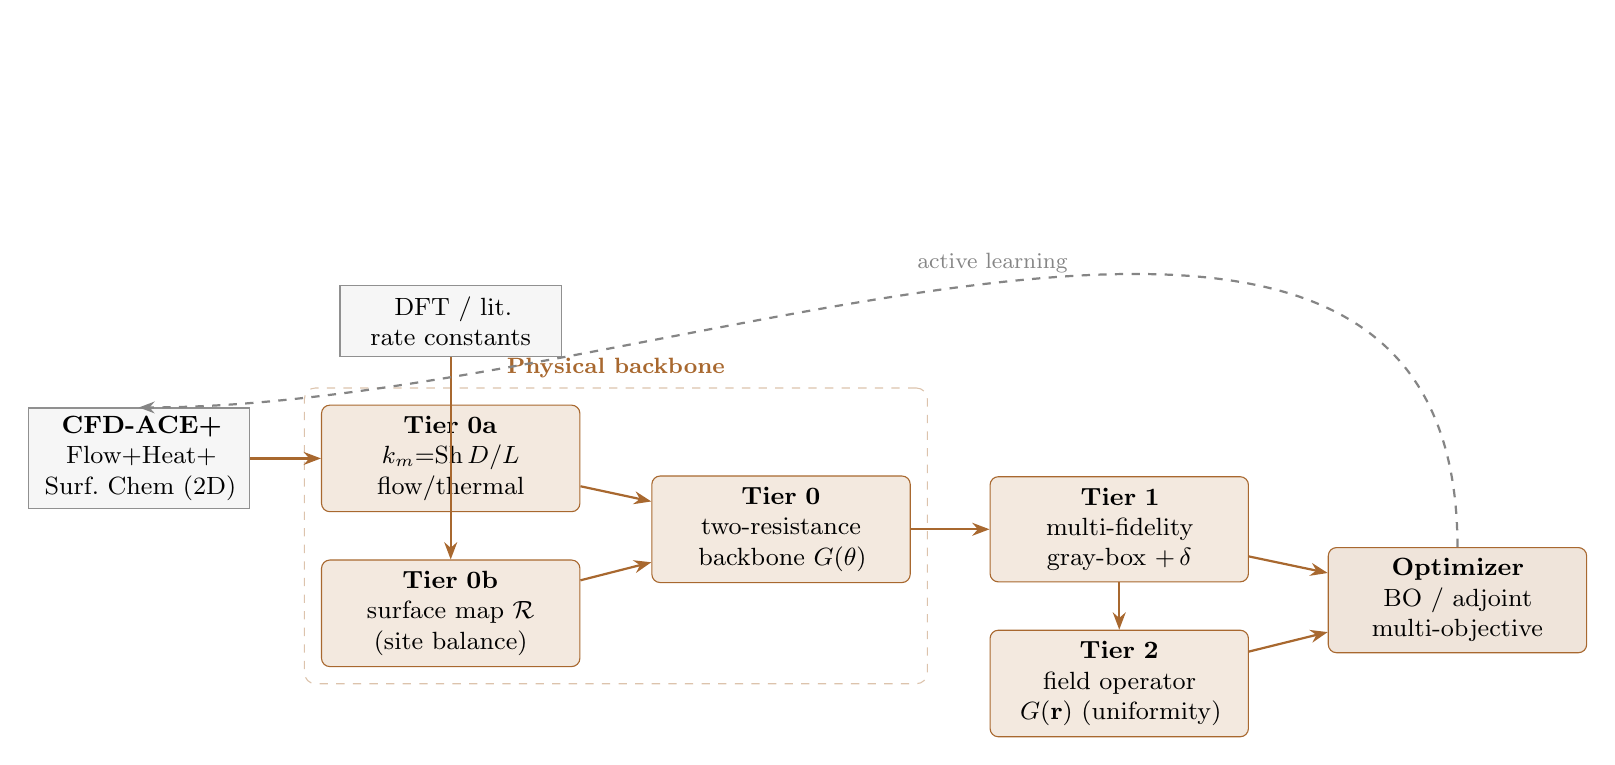
\begin{tikzpicture}[
  font=\small,
  node distance=6mm,
  box/.style={rectangle,rounded corners=3pt,draw=accent,fill=lightaccent,
    text width=3.0cm,minimum height=1.05cm,align=center,inner sep=4pt},
  data/.style={rectangle,draw=ink!50,fill=ink!4,text width=2.6cm,
    minimum height=0.9cm,align=center,inner sep=3pt},
  arr/.style={-{Stealth[length=2.2mm]},thick,accent},
  darr/.style={-{Stealth[length=2.0mm]},thick,ink!55,dashed}]

\node[data] (ace) {\textbf{CFD-ACE+}\\Flow+Heat+\\Surf.\ Chem (2D)};
\node[box,right=9mm of ace] (km) {\textbf{Tier 0a}\\$k_m{=}\Sh\,D/L$\\flow/thermal};
\node[box,below=6mm of km] (rk) {\textbf{Tier 0b}\\surface map $\R$\\(site balance)};
\node[box,right=9mm of km,yshift=-9mm] (tr) {\textbf{Tier 0}\\two-resistance\\backbone $G(\theta)$};
\node[box,right=10mm of tr] (gb) {\textbf{Tier 1}\\multi-fidelity\\gray-box $+\,\delta$};
\node[box,below=6mm of gb] (op) {\textbf{Tier 2}\\field operator\\$G(\mathbf r)$ (uniformity)};
\node[box,right=10mm of gb,yshift=-9mm,fill=accent!18] (opt) {\textbf{Optimizer}\\BO / adjoint\\multi-objective};

\node[data,above=6mm of km] (lit) {DFT / lit.\\rate constants};

\begin{scope}[on background layer]
\node[draw=accent!40,dashed,rounded corners,fit=(km)(rk)(tr),inner sep=6pt,
  label={[accent,font=\footnotesize\bfseries]above:Physical backbone}] {};
\end{scope}

\draw[arr] (ace) -- (km);
\draw[arr] (lit) -- (rk);
\draw[arr] (km) -- (tr);
\draw[arr] (rk) -- (tr);
\draw[arr] (tr) -- (gb);
\draw[arr] (gb) -- (op);
\draw[arr] (gb) -- (opt);
\draw[arr] (op) -- (opt);
\draw[darr] (opt) to[out=90,in=0] node[above,midway,font=\footnotesize]{active learning} (ace.north);
\end{tikzpicture}%
}
\caption{Pipeline. The physical backbone (Tier 0) is the prior; ACE+ data corrects it (Tier 1) and, when spatial uniformity matters, an operator surrogate (Tier 2) supplies $G(\mathbf r)$. The optimizer closes the loop, requesting new ACE+ runs only where they reduce decision uncertainty.}
\end{figure}

\subsection{Tier 1 --- multi-fidelity gray-box (the recommended workhorse)}
Treat the backbone as a cheap low-fidelity model $f_{\text{LF}}=G_{\text{backbone}}(\theta)$ and ACE+ as the expensive high-fidelity truth $f_{\text{HF}}$. Fuse them with an autoregressive multi-fidelity GP (Kennedy--O'Hagan):
\begin{equation}
f_{\text{HF}}(\theta)=\rho\,f_{\text{LF}}(\theta)+\delta(\theta),\qquad
\delta\sim\mathcal{GP}\!\big(m_\delta,\,k_\delta\big),
\end{equation}
so the GP only has to learn the (small, smooth) discrepancy $\delta$, not the whole response. This is dramatically more data-efficient than a stand-alone GP on $f_{\text{HF}}$, and it inherits the backbone's correct asymptotics --- so it \emph{extrapolates} in $T_s,p$ in a way a pure black box cannot. The same calibration step can fit unknown surface parameters (effective sticking coefficients, an effective $k_m$ prefactor) by Bayesian inference against ACE+, turning the surrogate-fitting into physical parameter estimation.

\subsection{Tier 2 --- field / operator surrogate (only if you need uniformity maps)}
Within-wafer nonuniformity is a \emph{field} quantity; a scalar surrogate cannot represent it. Two routes:
\begin{itemize}[leftmargin=1.4em,itemsep=2pt]
\item \textbf{Operator learning.} Train a DeepONet or Fourier Neural Operator to map (geometry parameters, inlet/thermal BCs) $\mapsto$ near-wall concentration field or directly $G(\mathbf r)$. DeepONet/FNO are designed for exactly this parametric-PDE-to-field setting and, with geometry inputs, transfer across designs; physics-informed DeepONet variants add PDE residual penalties so fewer ACE+ snapshots are needed.
\item \textbf{Projection ROM.} POD/PCA the passive-scalar snapshots, then learn the reduced dynamics by \emph{operator inference} (Peherstorfer--Willcox) --- a non-intrusive, polynomial-structured ROM that respects the advection--diffusion form. Cheaper and more interpretable than a neural operator when the field is smooth (which laminar RP-CVD fields are).
\end{itemize}
Because the precursor is a passive scalar on a frozen $(\uv,T)$ field, you can build the operator surrogate on the \emph{transport problem alone} and attach the surface BC analytically --- a big reduction in what the network must learn.

\subsection{Tier 0b detail --- if you ever do want to emulate stiff transients}
Should a later project need coverage transients (pulsed/cyclic), the modern tool is a neural \emph{operator} for stiff kinetics: DeepONet/flexDeepONet (Goswami et al.), partition-of-unity and Fourier-operator variants (EFNO, AMORE) learn the solution propagator of stiff reaction ODEs with flow-scale time steps and generalize to unseen initial states. Note this is overkill for the steady map $\R$ --- listed here only to mark the upgrade path.

\section{The optimization layer}
\label{sec:opt}

Define the QoIs over the operating vector $\theta=(T_s,\,p,\,\dot m,\,\{X_i\}_{\text{prec}},\,\{X_{\ce{HCl}}\dots\},\,\text{rotation})$ and geometry $g$:
\begin{gather}
\bar G(\theta)\ \text{(mean rate)},\qquad
\mathcal{U}(\theta)=\frac{\max_{\mathbf r}G-\min_{\mathbf r}G}{2\bar G}\ \text{(nonuniformity)},\notag\\[2pt]
\eta(\theta)=\frac{\text{Si deposited}}{\text{Si supplied}}\ \text{(utilization)},\qquad
\mathcal{S}\ \text{(selectivity)} .
\end{gather}
These trade off: pushing $\bar G$ up (more flux, higher $T$) usually worsens $\mathcal U$ and $\eta$. So the right target is a \textbf{Pareto front}, not a single optimum. Match the optimizer to the tier:

\begin{itemize}[leftmargin=1.4em,itemsep=3pt]
\item \textbf{Backbone/gray-box is differentiable} $\Rightarrow$ use \emph{gradient-based} optimization. You cannot autodiff through ACE+, but you \emph{can} autodiff through the reduced backbone (it is a handful of algebraic equations + a root-find; JAX with implicit-function-theorem differentiation through the $\dot s_j=0$ solve gives exact $\partial G/\partial\theta$). For field objectives on a Tier-2 ROM, an \emph{adjoint} gives the uniformity gradient cheaply. This is where your JAX skills pay off --- on the \emph{reduced} model, where AD is tractable, rather than on the full multiphysics, where it is not.
\item \textbf{GP surrogate (Tier 1/3)} $\Rightarrow$ \emph{Bayesian optimization}. Single objective: EI/UCB. Spec constraints (e.g.\ $\mathcal U\le 2\%$): constrained EI. Multi-objective Pareto: \texttt{qNEHVI} (BoTorch) or NSGA-II. \emph{Multi-fidelity BO} lets the acquisition function spend cheap backbone evaluations liberally and expensive ACE+ runs sparingly.
\item \textbf{Active learning to site ACE+ runs.} Don't pre-sample a fixed LHS grid and hope. Use the GP posterior variance (or an ISMO-style iterative scheme) to place each new ACE+ run where it most reduces uncertainty \emph{about the optimum/Pareto front} --- typically an order of magnitude fewer runs than space-filling DoE for the same decision quality.
\end{itemize}

\section{ACE+ workflow and design of experiments}
\label{sec:workflow}

The non-obvious discipline: \textbf{extract physics from each ACE+ run, not just the scalar QoI.} Every solve should yield, in addition to $G(\mathbf r)$: near-wall partial pressures $p_{i,s}(\mathbf r)$, wall fluxes $N_k$, the implied $\Sh$, boundary-layer thickness, and a local $\Da$ field. These feed the structured surrogate and let you verify the regime assumptions \emph{from the same runs} you use to fit.

\begin{center}
\renewcommand{\arraystretch}{1.25}
\begin{tabular}{@{}p{3.5cm} p{6.0cm} p{4.5cm}@{}}
\toprule
\textbf{Stage (2D first)} & \textbf{Runs / action} & \textbf{Output consumed by} \\
\midrule
A. Regime scoping & 6--10 corner+center points of the operating box; passive-scalar + flow/thermal only & Regime checklist (Sec.~\ref{sec:regime}); $\Sh(\Rey,\Sc)$ fit \\
B. Backbone assembly & none (assemble Tier 0 from A $+$ mechanism) & differentiable $G(\theta)$ \\
C. Gray-box calibration & 30--80 \emph{adaptively chosen} full runs & multi-fidelity GP $\delta$; calibrated $k_m$, sticking \\
D. Field surrogate (opt.) & $10^2$--$10^3$ snapshots if uniformity is a target & DeepONet/FNO or POD-OpInf for $G(\mathbf r)$ \\
E. Optimization & evaluate surrogate; confirm $\le$10 candidate optima in ACE+ & Pareto front; recipe \\
\bottomrule
\end{tabular}
\end{center}

\paragraph{Operating-space variables to sweep.} Susceptor/wafer temperature $T_s$; chamber pressure $p$; total flow / inlet velocity (sets $\Rey$, hence $k_m$); precursor mole fractions (\ce{SiH4} or \ce{SiH2Cl2}); for selective epi, \ce{HCl} fraction; carrier \ce{H2} split; and geometry features (gap height, inlet width, susceptor length, rotation rate). Use Sobol sequences for the initial space-filling set (better high-dimensional coverage than plain LHS), then switch to active learning.

\section{From 2D to 3D}
\label{sec:2dto3d}

Your 2D-first instinct is right and the pipeline is built to make the transition cheap rather than a restart:
\begin{enumerate}[leftmargin=1.4em,itemsep=2pt]
\item In 2D (axisymmetric or planar), validate the regime, fit $\Sh$, build and calibrate Tiers 0--1. The surface map $\R$ is geometry-\emph{independent} --- it transfers to 3D unchanged. That alone is a large head start, since the chemistry is the expensive-to-characterize part.
\item Treat 2D as a \emph{lower fidelity} of 3D in a multi-fidelity GP: a handful of 3D runs correct the 2D-fitted surrogate, rather than rebuilding from scratch. For the field surrogate, geometry-parametrized operator nets (and transfer learning / fine-tuning of a 2D-pretrained DeepONet onto 3D) keep the 3D data budget small.
\item Only genuinely 3D effects --- azimuthal flow nonuniformity from inlet/showerhead asymmetry, rotation, 3D buoyant rolls --- require new high-fidelity data; the backbone already carries everything that is dimension-agnostic.
\end{enumerate}

\section{Pitfalls and validation}
\label{sec:pitfalls}

\begin{itemize}[leftmargin=1.4em,itemsep=2pt]
\item \textbf{Soret diffusion is not negligible.} Light \ce{H2} mixtures show strong thermal diffusion; dropping the $D_k^T\nabla\ln T$ term in \eqref{eq:flux} biases near-wall concentration and hence $G$. Keep it on in ACE+ and (at least as a correction) in the backbone.
\item \textbf{Gas-phase chemistry sneaks back in.} The ``no volumetric reaction'' assumption fails if $T$/residence time let \ce{SiH4} pyrolyze or DCS decompose homogeneously. Monitor $\Da_{\text{gas}}$; if it grows, you must add a minimal gas-phase sub-mechanism (and your surrogate's passive-scalar premise weakens).
\item \textbf{Buoyancy and recirculation} break the stagnation-flow similarity and create nonuniformity the scalar surrogate won't see --- check $\Gr/\Rey^2$; if order one, you need the field tier.
\item \textbf{Rarefaction at RP.} Verify $\Kn$; add slip BCs if features are small / pressure low.
\item \textbf{Surrogate extrapolation.} GP/NN tiers must carry and respect uncertainty; never trust them outside the training box. The physical backbone is your guard-rail --- prefer the gray-box precisely because it degrades gracefully.
\item \textbf{Validation protocol.} Hold out ACE+ runs never used in fitting; report error on $G$, $\mathcal U$, $\eta$; confirm predicted optima in ACE+ before believing them; track calibrated physical parameters against literature/DFT values as a sanity check.
\end{itemize}

\section*{Recommended end-to-end path (the short version)}
\addcontentsline{toc}{section}{Recommended path}
\begin{keybox}
\begin{enumerate}[leftmargin=1.5em,itemsep=2pt]
\item \textbf{Scope the regime} with $\sim$8 ACE+ 2D runs; confirm $\Da\ll1$, dilute, $\Da_{\text{gas}}\ll1$; fit $\Sh(\Rey,\Sc,\text{geom})$.
\item \textbf{Assemble the differentiable backbone}: two-resistance coupling of $k_m$ with the steady surface map $\R$ (silane H-desorption model, or DCS with \ce{HCl}). Zero extra ACE+ cost.
\item \textbf{Gray-box it}: multi-fidelity GP learns the small ACE+ residual $\delta$ and calibrates sticking/$k_m$ ($\sim$30--80 adaptive runs).
\item \textbf{Add a field operator surrogate} (DeepONet/FNO or POD-OpInf) \emph{only if} within-wafer uniformity is an explicit objective.
\item \textbf{Optimize}: gradient/adjoint on the differentiable model for local refinement; multi-objective Bayesian optimization (\texttt{qNEHVI}) for the rate--uniformity--utilization Pareto front; active learning to place ACE+ runs.
\item \textbf{Lift to 3D} via multi-fidelity fusion (2D = low fidelity) and transfer-learned operators; $\R$ carries over unchanged.
\item \textbf{Keep pure LHS + GP black-box as the fallback and independent validator} --- never the primary model.
\end{enumerate}
\end{keybox}

\section*{Key references (by role in the pipeline)}
\addcontentsline{toc}{section}{References}
\footnotesize
\textbf{Stagnation/rotating-disk reduction \& reacting-flow theory.}
Coltrin, Kee, Evans, ``A mathematical model of the fluid mechanics and gas-phase chemistry in a rotating-disk CVD reactor,'' \emph{J.\ Electrochem.\ Soc.} \textbf{136}(3), 819--829 (1989);
Coltrin, Kee, Evans, Meeks, Rupley, Grcar, \textsc{Spin} (v3.83), Sandia SAND91-8003 (1991);
Kee, Coltrin, Glarborg, \emph{Chemically Reacting Flow: Theory and Practice} (Wiley, 2003/2017), ch.\ 7 (Stagnation Flows);
Kleijn et al., CVD benchmark vs.\ \textsc{Spin}, \emph{Thin Solid Films} (2000).

\textbf{Surface kinetics formalism \& Si epitaxy chemistry.}
Coltrin, Kee, Rupley, ``Surface Chemkin,'' \emph{Int.\ J.\ Chem.\ Kinet.} \textbf{23}, 1111--1128 (1991);
Sturm et al.\ (Princeton), H-desorption-limited Si CVD growth (review/data);
DFT of \ce{SiH4} adsorption / \ce{H2} desorption barrier $\approx$\,\SI{2.4}{eV} on \ce{Si}(001), \emph{Appl.\ Surf.\ Sci.} (2020);
modeling of \ce{SiH2Cl2} epitaxy with \ce{HCl}-desorption-limited low-$T$ regime, \emph{J.\ Cryst.\ Growth} (kinetics+transport).

\textbf{Surrogates \& optimization.}
Kennedy \& O'Hagan, multi-fidelity / Bayesian calibration (2000--2001);
Peherstorfer \& Willcox, operator inference ROM, \emph{CMAME} \textbf{306}, 196--215 (2016);
Lu, Jin, Karniadakis, DeepONet, \emph{Nat.\ Mach.\ Intell.} \textbf{3}, 218--229 (2021);
Li et al., Fourier Neural Operator, ICLR 2021;
Goswami et al., extended DeepONet for stiff chemical kinetics, \emph{CMAME} (2023);
Lye, Mishra, Ray, ISMO active learning for PDE-constrained optimization, \emph{CMAME} \textbf{374}, 113575 (2021);
GP-Bayesian-optimization of CVD process recipes (e.g.\ solar-thermal graphene CVD; semiconductor-equipment multi-fidelity surrogate studies).
\normalsize

\end{document}
